%------------------------------------------------------------------------------------------------
%
% LaTeX document Tally
%
%------------------------------------------------------------------------------------------------

\documentclass[11pt,a4paper]{article} % weitere Option: twoside

%------------------------------------------------------------------------------------------------

% weitere Pakete laden
        % Kodierung einstellen
\usepackage[ngerman]{babel}
\usepackage[T1]{fontenc}
\usepackage{graphicx}
\usepackage{ngerman}
\usepackage{listings}
\usepackage{color}
\usepackage[utf8x,utf8]{inputenc}



\definecolor{dkgreen}{rgb}{0,0.6,0}
\definecolor{gray}{rgb}{0.5,0.5,0.5}
\definecolor{mauve}{rgb}{0.58,0,0.82}

\lstset{numbers=left,
	numberstyle=\tiny,
	numbersep=5pt,
	breaklines=true,
	showstringspaces=false,
	frame=l ,
	xleftmargin=15pt,
	xrightmargin=15pt,
	basicstyle=\ttfamily\scriptsize,
	stepnumber=1,
	keywordstyle=\color{blue},          % keyword style
  	commentstyle=\color{dkgreen},       % comment style
  	stringstyle=\color{mauve}         % string literal style
}






% weitere Formatierung
\frenchspacing                         % Kein zus�tzlichen Abstand nach Punkt (.)
\setlength{\parindent}{0cm}            % keine Einr�ckung bei Beginn eines Absatzes
\setlength{\parskip}{1.5ex plus 0.5ex minus 0.5ex}  % mehr Absatzabstand


%------------------------------------------------------------------------------------------------
%
%  AB HIER SOLLEN �NDERUNGEN VORGENOMMEN WERDEN
%
%------------------------------------------------------------------------------------------------

% Hier sucht man sich den gew�nschten Stil f�r Kopf- bzw. Fu�zeile aus.
%\pagestyle{empty}                     % keine Kopf- und Fu�zeilen
\pagestyle{plain}                      % nur Seitenzahlen
%\pagestyle{headings}                  % Aktivieren f�r Kopf- und Fu�zeilen



\title{\normalfont\bfseries{Tally\\ digitale Strichliste am Raspberry Pi}\\---}
\author{Nicolai Tegtmeier \\ Dominik Scheffler \\ Philipp Frieling \\ Sebastian Reinke}
\date{23.06.2015}


%------------------------------------------------------------------------------------------------

\begin{document}

%------------------------------------------------------------------------------------------------

%\maketitle  % Titel erzeugen, verwendet die Angaben aus \title, \author und \date

%\tableofcontents % Um Inhaltsverzeichnis zu erzeugen

\begin{titlepage}
	\maketitle
	\begin{figure}[h]
	\makebox[\textwidth]{
	
\includegraphics[width=15cm]{TallyLogo.png}}
	\caption{Tally Logo}
	\end{figure}
\end{titlepage}
%------------------------------------------------------------------------------------------------

\tableofcontents
\newpage

\section{Projektvorfeld}
\label{Grundlagen}


\subsection{Kaffeestrichliste bisher}

In kleineren Unternehmen und Arbeitsgruppen gibt es oft einen zentralen Kaffee/ Getr\"anke -automaten und Snacks, an denen sich jeder Mitarbeiter bedienen kann. Um die Getr\"anke und Snacks kaufen zu k\"onnen wird meistens eine Strichliste auf Papier, meist in der N\"ahe des Automaten oder der Snacks, angebracht damit sich jeder Mitarbeiter eintragen kann, was er gekauft hat. Diese Liste wird oft zur besseren Verwaltung in eine Datenbank oder Tabelle eingepflegt, damit der Administrator einsehen kann wer wie viel gekauft hat. Hier passiert es jedoch h\''aufig das die Strichliste sehr unleserlich wird und es bei der \"Ubertragung in die Datenbank auf den PC zu Fehlern kommt. Au/ss{}erdem ist diese Methode f\"ur den Verantwortlichen sehr zeitaufwendig da alles per Hand \''ubertragen werden muss.
\par
Um diesem Problem entgegen zu wirken erarbeiten wir eine neue Methode um diese Daten 'digital' und einfacher speichern zu k\"onnen.
\cite{ahu61}
%------------------------------------------------------------------------------------------------

\section{Rahmenbedingungen}


\subsection{Aufgabe - die neue Kaffeestrichliste}
\label{SchriftAnpassen}

Um eine m\"oglichst energiesparende und handliche L\"osung zu finden, sollte die neue Strichliste auf einem Raspberry Pi 2 realisiert werden. Zun\"achst soll eine passende Benutzeroberfl\"ache f\"ur den Raspberry entwickelt werden, damit der Benutzer am Raspberry selber seine Eink\"aufe verbuchen kann. Dies soll mithilfe der integrierten Entwicklungsumgebung 'Qt Creator', die besonders zur Entwicklung von plattformunabh\"angigen C++ Programmen gedacht ist, entwickelt werden.
\par
Mithilfe eines Webservers, der ebenfalls auf dem Raspberry l\"auft, soll die Administration von jedem Computer im selben Netzwerk \"uber eine Weboberfl\"ache m\"oglich sein. Hier sollen auch die Benutzer ihre Daten einsehen und \"andern k\"onnen. Dazu wird eine MySQL/ SQLite Datenbank, sowie PHP Unterst\"utzung ben\"otigt. Mittels eines Barcodescanners soll es m\"oglich sein am Raspberry Produkte ein zu scannen.


\section{Ziele des Projekts}
Die neue 'digitale Kaffeestrichliste' wird auf Basis eines Raspberry Pi 2 entwickelt, um die alte Strichliste abzul\"osen. Dazu wurden folgende zu erreichende Ziele festgelegt:
\subsection{Zielbestimmung}
\label{Ausrichtung}

\subsubsection{Der Benutzer Account}
\"Uber den Benutzer Account soll der Benutzer sich am Raspberry selbst und an der Weboberfl\"ache anmelden k\''onnen. Am Raspberry selbst k\"onnen Getr\"anke und Snacks gekauft werden. Mithilfe der Weboberfl\"ache kann der Benutzer Statistiken einsehen und sein Passwort \"andern.

\subsubsection{Das Programm}
Das Programm das auf dem Raspberry l\"auft aktualisiert die Anzahl der Produkte im Lagerbestand automatisch, gibt Meldungen bei zu geringem Warebestand aus und gibt generelle Fehlermeldungen aus.

\subsubsection{Der Administrator Account}
Die Administration mithilfe des Administrator Accounts findet ausschliesslich \"uber die Weboberfl\"ache statt. Hier kann der Administrator Accounts hinzuf\"ugen und verwalten, Waren hinzuf\"ugen und verwalten und den Lagerbestand verwalten.

\subsection{Produkteinsatz}
\subsubsection{Anwendungsbereiche}
Mitarbeiter, beziehungsweise die Administratoren, k\"onnen eine Strichliste 'digital' anlegen. Diese fasst den zu bezahlenden Betrag f\"ur die Mitarbeiter zusammen.

\subsubsection{Zielgruppen}
Personengruppen und Unternehmen bei denen Getr\"anke und Snacks privat f\"ur alle angeboten und privat bezahlt werden, jedoch Schwierigkeiten mit der Handhabung einer herk\"ommlichen Strichliste haben und den Bestand an Getr\"anken und Snacks erfassen wollen.

\subsubsection{Betriebsbedingungen}
Die Strichliste soll m\"o
glichst Wartungsarm und einen niedrigen Stromverbrauch haben. Desweiteren soll sie t\"aglich vierundzwanzig Stunden laufen.

\subsection{Produktumgebung}
Das Produkt kann unabh\"angig an jedem Ort betrieben werden, solange eine Stromquelle in der n\"ahe ist.

\subsubsection{Software}
Die einzige Software die vom Benutzer ben\"otigt wird ist ein aktueller Webbrowser.

\subsubsection{Hardware}
Der Benutzer kann mit jedem Internetf\"ahigen Ger\"at die Weboberfl\"ache erreichen.

\subsubsection{Orgware}
Der Administrator kann die Betriebsparameter konfigurieren.

\subsection{Produktfunktion}
\subsubsection{Benutzerfunktion}
Ein im System registrierter Benutzer kann das System erst nutzen, wenn er angemeldet ist.
Nur ein Administrator kann einen Benutzer anlegen und ihm einen Benutzernamen sowie Passwort zuwesien. Sobald ein Benutzer registriert ist kann er sich sowohl am Raspberry als auch an der Weboberfl\"ache anmelden. Daf\"ur ben\"otigt er seinen Benutzernamen und sein Passwort. Abmelden ist bei beiden Oberfl\"achen jederzeit m\"oglich.
\par
Der Administrator kann \"uber die Weboberfl\"ache Produkte hinzuf\"ugen,entfernen und deren Details \"andern. Benutzer k\"onnen \"uber die Weboberfl\"ache Favoriten einrichten und Statistiken einsehen.
\par
Am Raspberry kann der registrierte und angemeldete Benutzer ein Produkt aus einer Liste w\"ahlen oder mithilfe eines Barcodescanners ein Prdoukt einscannen, welches im Warenkorb erscheint. Desweiteren kann er die Anzahl der Produkte erh\"ohen und seinen gesamten Warenkorb einsehen. Wenn er alle Waren im Warenkorb hat, kann er zur Kasse und die Waren durch einen Klick bezahlen, wodurch sein Konto belastet wird. Ein Abbruch oder das erreichen des Hauptmen\"us ist jederzeit m\"oglich.

\subsection{Programmfunktion}
Beim Kauf eines Produktes aktualisiert das Programm automatisch den Warenbestand. Bei geringem Warenbestand wird eine Warnmeldung ausgegeben und bei fehlen des Artikels wird dieser entfernt.

\subsection{Serverfunktion}
Auf dem Raspberry soll ein Apache 2 Server mit PHP Unterst\"utzung laufen.
\subsubsection{Datenbank}
Als Datenbank soll die resourcenschonendere SQLite Datenbank verwendet werden

\subsection{Benutzerschnittstelle}
Die Bedienung des Raspberry erfolgt \"uber einen eingebauten Touchscreen am Raspberry. Au\ss()erdem wird ein Barcodescanner installiert um Produkte einscannen zu k\"onnen.

\begin{center}
\begin{large}
\textbf{Zentrierter Text hingegen ist schon eher nützlich.}
\end{large}
\end{center}


\section{Meilensteine des Projektes}
\label{Meilensteine}

\subsection{Raspberry Pi 2 Model B - Die Hardware mit der passenden Software}
Mit dem Raspberry Pi 2 war schon im Projektvorfeld eine passende Basis f\"ur das Projekt gegeben. Der Raspberry Pi 2 besitzt einen Vierkern ARM Cortex-A7 Prozessor mit jeweils 900MHz und einen Gigabyte ARbeitsspeicher. Desweiteren befinden sich vier USB 2.0 Ports, eine 40 GPIO pin Steckerleiste, ein HDMI Anschluss, ein Ethernet Port und ein Micro SD Kartenslot am Raspberry.
\par
Ausser dem Raspberry Pi 2 war zun\"achst ein 3,5 Zoll Touchscreen der Firma admatec \cite{zitat01} mit dem Namen C-Berry Touch vorhanden, das mittels eines Adapterboards an der GPIO Stiftleiste des Raspberry angesteckt wird. Das Display besitzt eine Aufl\"osung von 320x240 Pixeln, eine LED- Hintergrundbeleuchtung und wird komplett vom Raspberry mit Strom versorgt.

	\begin{figure}[h]
	\makebox[\textwidth]{
	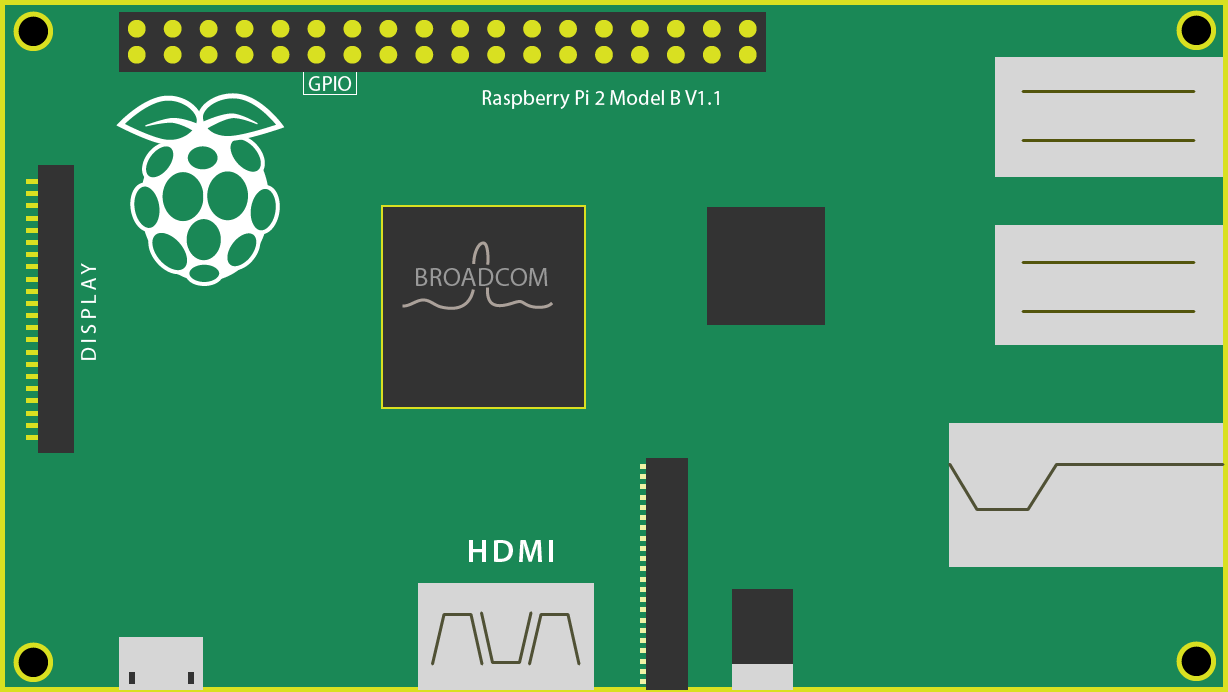
\includegraphics[width=9cm]{RaspberryPi.png}}
	\caption{Der Raspberry Pi 2}
	\end{figure}
\newpage
\par
\subsubsection{Betriebssystem und Verbindung zu anderen Rechnern}
Als erster Schritt wurde nach einem passenden Betriebssystem gesucht. Von Anfang an stand fest das ein Linuxderivat auf dem Raspberry laufen sollte. Hierbei fiel die Wahl auf das speziell f\''ur den Raspberry optimierte Debianderivat `Raspbian'.
\par
'Raspbian' wurde so optimiert das es mit der geringen Hardware zurecht kommt und den ARM-Prozessor des Raspberrys unterst\''utzt. Als Alternative stand eine Ubuntu Version ,speziell f\"ur ARM-Prozessoren entwickelt, zu Verf\"ugung die jedoch noch nicht voll ausgereift und funktionst\''uchtig ist.
\par
 Um die weitere Einrichtung des Raspberrys zu vereinfachen wurde, neben der vorkonfigurierten und installierten SSH Verbindung zur Verwaltung \"uber ein Konsolenprogramm (Windows: Putty), eine freie Implementierung des Remote Desktop Protocols f\"ur Linux Names 'xrdp' installiert.
\begin{frame}

\begin{lstlisting}
sudo apt-get install xrdp
\end{lstlisting}

\end{frame}
Damit ist eine einfache Remote Desktopverbindung zum Raspberry m\"oglich und die komplette Verwaltung kann \''uber einen Windows, Mac oder Linux Computer erfolgen. 
\par
\subsubsection{Der Webserver}
Als n\"achster Schritt wurde ein vollst\"andiger Webserver auf dem Raspberry eingerichtet. Hierzu wurde zun\"achst ein Apache Server der Version 2 installiert
\begin{frame}

\begin{lstlisting}
sudo apt-get install apache2
\end{lstlisting}

\end{frame}
 der \"uber eine hohe Stabilit\"at und Geschwindigkeit verf\"ugt und serverseitig die Skriptsprache PHP unterst\"utzt. Im Anschluss wurde das PHP5 Paket installiert
 \begin{frame}

\begin{lstlisting}
sudo apt-get install php5
\end{lstlisting}

\end{frame}
 um eine volle Unterst\"utzung f\"ur die kommende Websites zu gew\"ahrleisten.
 \par
 PHP ist eine Open Source-Skriptsprache die speziell f\''ur die Webprogrammierung geeignet ist. Wenn eine Anfrage an die Website gestellt wird, wird der PHP-Code auf dem Server ausgef\''uhrt und erzeugt eine HTML-Ausgabe die dann letztendlich an den Client gesendet wird.
\par
\subsubsection{Die passende Datenbank}
Nun stand die Auswahl des passenden Datenbankverwaltungssystems an. Zur Auswahl standen die Systeme MySQL und SQLite. Bei Recherchen zu den beiden Datenbanken stellte sich schnell heraus das die MySQL Datenbank zwar auf dem Raspberry lauff\"ahig ist aber keine hohe Stabilit\"at besitzt und sehr resourcenlastig auf dem Raspberry l\"auft. Daher wurde das SQLite Datenbanksystem ausgew\"ahlt.
\begin{frame}

\begin{lstlisting}
apt-get install sqlite3
apt-get install php5-sqlite
\end{lstlisting}

\end{frame}
 SQLite ist eine relationale Datenbank und ben\"otigt im Gegensatz zu MySQL keine st\"andig laufende Software da die Datenbank aus einer einzigen, wenigen Kilobyte grossen, Datei besteht. SQLite  legt Wert auf Geschwindigkeit und Einfachheit.
\par
\subsubsection{Der Touchscreen}
Als erstes wurde der Treiber für den bereitgestellte C-Berry Touchscreen installiert
\begin{frame}

\begin{lstlisting}
wget http://www.airspayce.com/mikem/bcm2835/bcm2835-1.36.tar.gz
tar zxvf bcm2835-1.36.tar.gz
cd bcm2835-1.36
./configure
make
sudo make check
sudo make install
\end{lstlisting}

\end{frame}
und im Anschluss die Beispielsoftware zum anzeigen von Bildern installiert
\begin{frame}

\begin{lstlisting}
wget http://admatec.de/sites/default/files/downloads/C-Berry.tar.gz
tar zxvf C-Berry.tar.gz
cd C-Berry/SW/tft_test
make
sudo ./tft_test
\end{lstlisting}

\end{frame}

Nach ersten Tests mit dem C-Berry Touchscreen fiel auf das es nicht als Prim\"ares Display geeignet ist, da vom Desktop ein Screenshot erstellt wird und dieser auf dem Display ausgegeben wird. Starke Verz\"ogerungen im Bildaufbau und eine schlechte Bedienung mithilfe des Touchscreens waren die Folge. Das Display ist mehr daf\''uhr gedacht andere Inhalte als den Desktop wiederzugeben, die dann per Touchscreen bedient werden wie zum Beispiel einzelne Buttons.
\par
Damit war der Touchscreen ungeeignet f\''ur das Projekt und ein neuer Touchscreen mit besserer Anbindung an den Rapsberry und einer h\"oheren Bildwiederholungsrate musste gesucht werden. Dabei kam die Idee auf, ein 7 Zoll resistives Touchscreen von Pollin zu verwenden das durch seine Gr\"osse viel Platz f\"ur das Tally Programm bietet und eine sehr gute Touch Bedienung verspricht. Von Vorteil war auch die eigene externe Grafikeinheit die eine hohe Bildwiederholungsrateerm\"oglicht  und ein externer USB- Touchcontroller der die Bedienung des Touchscreens besser ausf\''uhren soll.
\par
Jedoch stellte die externe Stromversorgung ein Problem dar, da man jeweils ein Stromkabel f\"ur den Raspberry und eins f\"ur das Display ben\"otigt, damit w\"are eine Energiesparende L\"osung ebenfalls nicht m\"oglich.
\par
Deshalb fiel die Entscheidung zugunsten des 3,5 Zoll Touchscreen 4DPi-35 von 4D System aus. Der Touchscreen besitzt eine Aufl\"osung von 480x320 Pixeln und durch die High Speed 48Mhz SPI Verbindung werden hohe und konstante Bildwiederholungsraten erm\"oglicht.
Die Vorteile bei diesem Display waren die kleine Bauform und keine zus\"atzlich ben\"otigte Stromquelle. Ausserdem wird vom Hersteller direkt ein passender Kernel f\"ur Raspbian zur Verf\"ugung gestellt.
\begin{frame}

\begin{lstlisting}
wget http://www.4dsystems.com.au /downloads/4DPi/kernel4dpi_1.3-3_pi2.deb 

sudo dpkg -i kernel4dpi_1.3-3_pi2.deb
\end{lstlisting}

\end{frame}

 Nachdem das erforderliche Paket installiert wurde, musste der Raspberry herunter gefahren werden,  das Display an den GPIO-Ports angebracht werden und der Raspberry wieder hoch gefahren werden. Danach war ein sofortiger Betrieb m\"oglich da der Raspberry das Display als prim\''ares Display erkennt und direkt auf den Desktop bootet. Dadurch ist kein HDMI Bildschirm mehr notwendig und die Bedienung kann ausschliesslich \"uber den Touchscreen erfolgen.
\par
\subsubsection{Produkte scannen}
Zur vereinfachten Eingabe von Produkten soll ausserdem ein Barcodescanner angebracht werden. Hier sollte entweder ein handesl\"ublicher Barcodescanner per USB an den Raspberry angeschlossen werden, der Barcode mittels USB Webcam und passender Software oder aber ein Barcodescannermodul an den GPIO's des Raspberry als Lösung dienen.
\par
 Da jedoch das ein Barcodescannermodul nur mit ca. drei Volt betrieben werden kann, der Raspberry aber ca. fünf Volt an den GPIO's zur Verf\"ugung stellt, wurde überlegt eine Webcam an den Raspberry anzuschliessen und mittels einer Software das Bild auf Barcodes zu untersuchen. Die Wahl fiel allerdings auf das Scannen mittels USB Barcodescanner, da dies eine einfacherere Handhabung mit verspricht und der Barcodescanner direkt als USB Tastatur erkannt wird.
\par
\subsubsection{Wlan für den Raspberry}
Damit am Raspberry nicht immer ein Patchkabel angeschlossen werden muss, wurde der Edimax WLAN USB Stick am Raspberry angeschlossen. Der Edimax WLAN Stick wird automatisch von Raspbian erkannt da schon alle erforderlichen Pakete und Treiber installiert sind, weshalb dieser WLAN Stick empfohlen wird falls man WLAN am Raspberry benutzen m\"ochte. Zun\"achst wurde in der automatische 'Power Saving' Modus abgeschaltet. Hierzu wurde eine Konfigurationsdatei f\"ur den Treiber des WLAN Sticks erstellt.
\begin{frame}

\begin{lstlisting}
sudo nano /etc/modprobe.d/8192cu.conf
\end{lstlisting}

\end{frame}
\par

mit folgendem Inhalt
\begin{frame}

\begin{lstlisting}
options 8192cu rtw_power_mgnt=0 rtw_enusbss=0
\end{lstlisting}

\end{frame}
\par
\par
Um nun eine Verbindung mit dem Wlan herzustellen wurde die folgende Datei
\begin{frame}

\begin{lstlisting}
sudo nano /etc/network/interfaces
\end{lstlisting}

\end{frame}

um folgenden Inhalt ergänzt
\begin{frame}

\begin{lstlisting}
auto lo
iface lo inet loopback
iface eth0 inet dhcp

auto wlan0
allow-hotplug wlan0
iface wlan0 inet dhcp
wpa-ap-scan 1
wpa-scan-ssid 1
wpa-ssid "WLAN-NAME"
wpa-psk "WLAN-PASSWORT"

\end{lstlisting}

\end{frame}

damit eine Verbindung mit dem WLAN Netz hergestellt werden kann.
Anschliessend muss nur noch per
\begin{frame}

\begin{lstlisting}
sudo service networking restart
\end{lstlisting}

\end{frame}
der Netzwerkdienst neu gestartet werden und eine Verbindung mit dem angegebenen WLAN Netz wird hergestellt.
\par
Da diese M\''oglichkeit jedoch relativ umst\''andlich ist und Linux Kenntnisse erfordert, wird in das Tally Programm eine einfache WLAN konfiguration eingebaut in der man den WLAN-Namen un das WLAN-Passwort eingeben kann um sich mit dem WLAN-Netz zu verbinden.

\subsubsection{angepasster Bootscreen}
Während eines Meetings kam die Idee auf den Bootscreen zu verändern und ein eigenes Bild w\''ahrend des hochfahrens anzuzeigen. Dazu wird eine weitere Software benötigt, der 'Frame Buffer Imageviewer', der ein Bild in den Speicherbuffer l\''adt das w\''ahrend des hochfahrens angezeigt werden kann.
\begin{frame}

\begin{lstlisting}
sudo apt-get install fbi
\end{lstlisting}

\end{frame}

Danach muss ein passendes Skript geschrieben werden welches das Bild beim booten anzeigt.
\begin{frame}

\begin{lstlisting}
sudo nano asplashscreen
\end{lstlisting}

\end{frame}

\begin{frame}

\begin{lstlisting}
#! /bin/sh
### BEGIN INIT INFO
# Provides:          asplashscreen
# Required-Start:
# Required-Stop:
# Should-Start:      
# Default-Start:     S
# Default-Stop:
# Short-Description: Show custom splashscreen
# Description:       Show custom splashscreen
### END INIT INFO
 
do_start () {
 
    /usr/bin/fbi -T 1 -noverbose -a /etc/splash.png    
    exit 0
}
 
case "$1" in
  start|"")
    do_start
    ;;
  restart|reload|force-reload)
    echo "Error: argument '$1' not supported" >&2
    exit 3
    ;;
  stop)
    # No-op
    ;;
  status)
    exit 0
    ;;
  *)
    echo "Usage: asplashscreen [start|stop]" >&2
    exit 3
    ;;
esac
 
:
\end{lstlisting}

\end{frame}

Dieses Skript wird nun in den passenden Ordner verschoben damit es beim Start ausgeführt werden kann
\begin{frame}

\begin{lstlisting}
sudo mv asplashscreen /etc/init.d/asplashscreen
\end{lstlisting}
\end{frame}

Als letztes wird das Skript für den Raspberry ausführbar gemacht und als Bootscript registriert
\begin{frame}

\begin{lstlisting}
sudo chmod a+x /etc/init.d/asplashscreen
sudo insserv /etc/init.d/asplashscreen
\end{lstlisting}
\end{frame}

Nun wird w\''ahrend des Bootvorgangs das Tally Logo angezeigt.

\subsubsection{Backups einrichten und versenden per Mail}
Als m\"ogliche Backupvarianten standen ein komplettes Backup der Speicherkarte des Raspberrys oder ein Backup der Datenbank zur Wahl.
\par
Der Entschluss fiel auf ein Backup der Datenbank, da diese auch per Mail an den jeweiligen Administrator geschickt werden soll. Dazu wird Rsync verwendet, das mit folgendem Befehl installiert wird:
\begin{frame}

\begin{lstlisting}
sudo apt-get install rsync
\end{lstlisting}
\end{frame}
 Rsync ist ein Programm das Dateien oder Ordner in verschiedenen Pfaden speichern kann. Dazu \"uberpr\"uft es zun\"achst ob die zu kopierende Datei ge\"ander wurde oder nicht, wodurch ein unn\"utzes kopieren von Daten unterbunden wird.
\par
Damit die backups autmatisch und t\"aglich erstellt werden, wird ein cronjob hinzugef\"ugt. Cronjobs, oder auch Cron-Daemon, ist ein Dienst um Skripte oder Programme zu einer bestimmten Zeit starten zu k\''onnen.
\begin{frame}

\begin{lstlisting}
sudo crontab -e
\end{lstlisting}
\end{frame}

Hier wird folgende Zeile eingef\"ugt
\begin{frame}

\begin{lstlisting}
rsync -a QUELLE ZIEL 
\end{lstlisting}
\end{frame}
Dadurch wird das Programm jeden Tag um .... aufgerufen und die Datenabank von ... nach ... kopiert.
\par
Diese Datei wird nun auch t\"aglich, nach dem erstellen des Backups, an den Admin per mail gesendet.
Daf\"ur wird das Programm sendEmail und zwei Perl- Libraries installiert. SendEmail hat den Vorteil das kein Mailserver auf dem Raspberry installiert werden muss und der Raspberry als ein eigener 'sende Client' erkannt wird. Die beiden Perl- Libraries dienen dazu damit eine verschl\"usselte Verbindung per TLS zum Mailserver aufgebaut werden kann.
\par
Zum autmatischen versenden der Mails wird folgendes Skript erstellt
\begin{frame}

\begin{lstlisting}
sudo nano /usr/local/bin/mailnotify.sh
\end{lstlisting}
\end{frame}
Das Skript sieht wie folgt aus
\begin{frame}

\begin{lstlisting}
###########################################################################
                                                                     												  
              Sending E-Mail notification with sendEmail              									 
                                                                      											 
 Creation:    15.08.2013                                              										 
 Last Update: 20.10.2013                                               										 
                                                                       											
 Copyright (c) 2013 by Georg Kainzbauer <http://www.gtkdb.de>          							
                                                                      											 
 This program is free software; you can redistribute it and/or modify 								 
 it under the terms of the GNU General Public License as published by								  
 the Free Software Foundation; either version 2 of the License, or    								 
 (at your option) any later version.                                   									
                                                                       											
###########################################################################
#!/bin/bash

# Sender of the mail
SENDER="absender@domain.de"

# Recipient of the mail
RECIPIENT="empfaenger@domain.de"

# SMTP server
SMTPSERVER="smtp.domain.de"

# User name on the SMTP server
SMTPUSERNAME="MeinMailAccount"

# Password on the SMTP server
SMTPPASSWORD="MeinMailPasswort"

# Enable TLS for the SMTP connection
USETLS=1

###################################################################
# NORMALLY THERE IS NO NEED TO CHANGE ANYTHING BELOW THIS COMMENT #
###################################################################

# Use first argument as mail subject
if [ -n "$1" ]; then
  SUBJECT="$1"
else
  # No subject specified
  SUBJECT=""
fi

# Use second argument as mail body
if [ -n "$2" ]; then
  BODY="$2"
else
  # No mail body specified
  BODY=""
fi

# Generate the options list for sendEmail
OPTIONS=""

if [ -n "${SMTPSERVER}" ]; then
  OPTIONS="${OPTIONS} -s ${SMTPSERVER}"
fi

if [ -n "${SMTPUSERNAME}" ]; then
  OPTIONS="${OPTIONS} -xu ${SMTPUSERNAME}"
fi

if [ -n "${SMTPPASSWORD}" ]; then
  OPTIONS="${OPTIONS} -xp ${SMTPPASSWORD}"
fi

if [ -n "${USETLS}" ]; then
  if [ ${USETLS} == 1 ]; then
    OPTIONS="${OPTIONS} -o tls=yes"
  else
    OPTIONS="${OPTIONS} -o tls=no"
  fi
fi

# Send the mail with sendEmail
sendEmail -f ${SENDER} -t ${RECIPIENT} -u "${SUBJECT}" -m "${BODY}" ${OPTIONS}

exit 0
\end{lstlisting}
\end{frame}

Zu editieren sind folgende Punkte:
\begin{frame}

\begin{lstlisting}
# Sender of the mail
SENDER="absender@domain.de"

# Recipient of the mail
RECIPIENT="empfaenger@domain.de"

# SMTP server
SMTPSERVER="smtp.domain.de"

# User name on the SMTP server
SMTPUSERNAME="MeinMailAccount"

# Password on the SMTP server
SMTPPASSWORD="MeinMailPasswort"
\end{lstlisting}
\end{frame}
Hier m\"ussen nur noch die Empf\"anger-Emai-Adresse und Absende-Email-Adresse mit dazugeh\"origem SMTP- Server, Benutzername und Passwort angegeben werden.
Danach muss das Skript ausf\"uhrbar gemacht werden
\begin{frame}

\begin{lstlisting}
sudo chmod +x /usr/local/bin/mailnotify.sh
\end{lstlisting}
\end{frame}

Im Anschluss kann die erste Email versendet werden
\begin{frame}

\begin{lstlisting}
mailnotify.sh "Test" "Dies ist eine Testnachricht."

\end{lstlisting}
\end{frame}
Damit wird das Skript aufgerufen, wobei der text in den ersten Anf\"uhrungszeichen den Betreff, un der zweite den Inhalt der Email.
Hierbei kam es jedoch zu folgendem Fehler
\begin{frame}

\begin{lstlisting}
invalid SSL_version specified at /usr/share/perl5/IO/Socket/SSL.pm line 332

\end{lstlisting}
\end{frame}

Dieser Fehler entsteht da die dazugeh\"orige SSL konfiguration einen kleinen Fehler enth\"ahlt.
Folgende Datei muss aufgerufen werden
\begin{frame}

\begin{lstlisting}
sudo nano /usr/share/perl5/IO/Socket/SSL.pm

\end{lstlisting}
\end{frame}

und in Zeile 1490 muss folgender Inhalt
\begin{frame}

\begin{lstlisting}
m{^(!?)(?:(SSL(?:v2|v3|v23|v2/3))|(TLSv1[12]?))$}i

\end{lstlisting}
\end{frame}

durch
\begin{frame}

\begin{lstlisting}
m{^(!?)(?:(SSL(?:v2|v3|v23|v2/3))|(TLSv1[12]?))}i

\end{lstlisting}
\end{frame}

ersetzt werden.Nur das Dollar Zeichen am Schluss muss entfernt werden. Anschliessend k\"onnen Emails versendet werden
\begin{frame}

\begin{lstlisting}
mailnotify.sh "Test" "Dies ist eine Testnachricht."
Jul 15 16:32:30 raspberrypi sendEmail[4163]: Email was sent successfully!

\end{lstlisting}
\end{frame}
\par
Damit auch Anh\"ange mit versandt werden k\"onnen muss lediglich das Skript etwas ver\"andert werden
Hinzu kommt folgender Ausdruck.
\begin{frame}

\begin{lstlisting}
# Use third argument as attachment
if [ -n "$3" ]; then
  ATTACHMENT="$3"
else
  # No attachment specified
  ATTACHMENT=""
fi

\end{lstlisting}
\end{frame}

Somit sieht das Skript wie folgt aus
\begin{frame}

\begin{lstlisting}
#!/bin/bash

# Sender of the mail
SENDER="absender@domain.de"

# Recipient of the mail
RECIPIENT="empfaenger@domain.de"

# SMTP server
SMTPSERVER="smtp.domain.de"

# User name on the SMTP server
SMTPUSERNAME="MeinMailAccount"

# Password on the SMTP server
SMTPPASSWORD="MeinMailPasswort"

# Enable TLS for the SMTP connection
USETLS=1

###################################################################
# NORMALLY THERE IS NO NEED TO CHANGE ANYTHING BELOW THIS COMMENT #
###################################################################

# Use first argument as mail subject
if [ -n "$1" ]; then
  SUBJECT="$1"
else
  # No subject specified
  SUBJECT=""
fi

# Use second argument as mail body
if [ -n "$2" ]; then
  BODY="$2"
else
  # No mail body specified
  BODY=""
fi

# Use third argument as attachment
if [ -n "$3" ]; then
  ATTACHMENT="$3"
else
  # No attachment specified
  ATTACHMENT=""
fi

# Generate the options list for sendEmail
OPTIONS=""

if [ -n "${SMTPSERVER}" ]; then
  OPTIONS="${OPTIONS} -s ${SMTPSERVER}"
fi

if [ -n "${SMTPUSERNAME}" ]; then
  OPTIONS="${OPTIONS} -xu ${SMTPUSERNAME}"
fi

if [ -n "${SMTPPASSWORD}" ]; then
  OPTIONS="${OPTIONS} -xp ${SMTPPASSWORD}"
fi

if [ -n "${USETLS}" ]; then
  if [ ${USETLS} == 1 ]; then
    OPTIONS="${OPTIONS} -o tls=yes"
  else
    OPTIONS="${OPTIONS} -o tls=no"
  fi
fi

if [ -n "${ATTACHMENT}" ]; then
  OPTIONS="${OPTIONS} -a ${ATTACHMENT}"
fi

# Send the mail with sendEmail
sendEmail -f ${SENDER} -t ${RECIPIENT} -u "${SUBJECT}" -m "${BODY}" ${OPTIONS}

exit 0
\end{lstlisting}
\end{frame}
Im Befehl zum senden wird nun ein drittes Argument hinzugef\"ugt das den Pfad mit der Datei die zu versenden ist enth\"alt.
\begin{frame}

\begin{lstlisting}
mailnotify.sh "Test" "Dies ist eine Testnachricht." anhang.tar.gz

\end{lstlisting}
\end{frame}

\subsubsection{Tally autostarten}
Damit nach dem starten des Raspberry Pi direkt das Tally Programm geladen wird musste der Autostart f\"ur das Programm konfiguriert werden.
\par
Die erste Idee war das Programm per cronjob nach jedem neuen hochfahren zu starten. Daf\"ur musste zun\"achst ein kleines Skript geschrieben werden damit das Programm autostarten kann, welches dann in einem cronjob nach jedem hochfahren ausgef\"uhrt wird.
\begin{frame}

\begin{lstlisting}
sudo nano /etc/init.d/NameDesSkripts
\end{lstlisting}
\end{frame}
\begin{frame}

\begin{lstlisting}
#! /bin/sh
### BEGIN INIT INFO
# Provides: NAME DES PROGRAMMES
# Required-Start: $syslog
# Required-Stop: $syslog
# Default-Start: 2 3 4 5
# Default-Stop: 0 1 6
# Short-Description:
# Description:
### END INIT INFO
 
case "$1" in
  start)
    echo "NAME DES PROGRAMMES wird gestartet"
    # Starte Programm
    /pfad/des/programmes
    ;;
  stop)
    echo "NAME DES PROGRAMMES wird beendet"
    # Beende Programm
    killall noip2
    ;;
  *)
    echo "Benutzt: /pfad/des/programmes {start|stop}"
    exit 1
    ;;
esac
 
exit 0
\end{lstlisting}
\end{frame}

Danach wird das Skript ausf\"uhrbar gemacht
\begin{frame}

\begin{lstlisting}
sudo chmod 755 /etc/init.d/NameDesSkripts
\end{lstlisting}
\end{frame}
Um zu testen ob das Skript auch richtig funktioniert wird es mit folgendem Befehl aufgerufen
\begin{frame}

\begin{lstlisting}
sudo /etc/init.d/NameDesSkripts start
\end{lstlisting}
\end{frame}

und wieder gestoppt
\begin{frame}

\begin{lstlisting}
sudo /etc/init.d/NameDesSkripts stop
\end{lstlisting}
\end{frame}

Damit der Raspberry das Skript beim booten l\"adt wird noch folgender Befehl ausgef\"uhrt der das Programm in den passenden Runlevel bringt
\begin{frame}

\begin{lstlisting}
sudo update-rc.d NameDesSkripts defaults
\end{lstlisting}
\end{frame}
\par

Als n\"achstes wird das Skript durch einen cronjob jedes mal beim starten des Raspberrys ausgef\"uhrt

\begin{frame}

\begin{lstlisting}
sudo crontab -e
\end{lstlisting}
\end{frame}
Dazu wurde folgende zeile eingef\"ugt
\begin{frame}

\begin{lstlisting}
@reboot \bin\bash .....
\end{lstlisting}
\end{frame}
Das '@reboot' steht f\"ur das ausf\"uhren der Datei nach jedem neuen hochfahren des Raspberry. Jedoch startete das Programm nach dem hoch fahren des Raspberrys nicht. Erst als die Konsole ge\"offnet wurde startete der cronjob das Skript und somit das Programm.
\par
Die beschriebene Methode war lediglich daf\"ur gedacht Programme auszuf\"uhren die keine GUI ben\"otigen. Alle Programme die autostarten sollen und eine GUI ben\"otigen m\"ussen \"uber die globale LXDE (Lightweight X11 Desktop Environment) Autostart funktion gestartet werden.
Dazu erstellt man in folgendem Pfad
\begin{frame}

\begin{lstlisting}
/etc/xdg/autostart/
\end{lstlisting}
\end{frame}
eine Datei die wie folgt lauten muss 'NamedesProgramm.desktop'. Wichtig ist das .desktop da sonst das Programm nicht nach dem hochfahren gestartet wird.
\begin{frame}

\begin{lstlisting}
[Desktop Entry]
Name=NamedesProgramm
Comment=
Exec=NamedesProgramm -forever -rfbport 5900 -rfbauth ~/.vnc/x11vnc.pass -o ~/.vnc/x11vnc.log -display :0
Terminal=false
Type=Application
\end{lstlisting}
\end{frame}

Diese Datei wieder ausf\"uhrbar machen
\begin{frame}

\begin{lstlisting}
chmod +x x11vnc.desktop
\end{lstlisting}
\end{frame}
Und das gew\"unschte Programm startet nachdem die GUI geladen ist.



\subsection{QT Creator - Das Tally programm}
Als Programmierumgebung, für den Raspberry Pi 2, wurde Qt gewählt.
Qt ist eine Klassenbibliothek von C++ und bietet die Programmierung für  graphische Benutzeroberfläche und Datenbankfunktionen.
Wir arbeiten mit der Version 4.8.1 von Qt, da neuere Versionen noch nicht mit dem Raspberry Pi 2 kompatibel sind.
Als Debugger haben wir GNU gdb 7.8 für MinGW 4.9.1 gewählt.
\par
Programmiert wird hauptsächlich auf einem PC, da dieser schneller debuggen kann.
Darüber hinaus musste der Raspberry PI 2 noch konfiguriert werden, wie in 4.1 beschrieben, wodurch ein zeitgleiches arbeiten erschwert wäre.
Es wurde sich darauf geeinigt das Programm zu Demonstrationszwecke, während den Teammeetings, auf dem Raspberry PI 2 laufen zu lassen.
Zum Ende des Projekts, sobald die Konfiguration beendet ist, sollten wir denn Raspberry PI 2 bekommen um die Benutzeroberfläche letztendlich anpassen zu können.
\par
\subsubsection{Die Benutzeroberfl\"ache}
Als erstes haben wir erste Grundzüge der Benutzeroberfläche thematisiert. Letztendlich haben wir eine herausgearbeitet, welche in dem Plichtenheft zu sehen ist.
Außerdem wurden mehrere Strukturen für das Hauptprogramm besprochen und haben uns auf einen Automaten geeinigt. Näheres dazu findet sich in dem Unterpunkt Aufbau des Programmes.
Daraufhin wurde sich in Qt eingelesen und die ersten Funktionen für den Login-Screen programmiert.
Wie bereits in Abschnitt 4.1 erklärt, wurde entschieden das Display zu wechseln.
Außerdem ist uns Aufgefallen das  sehr viele Klicks gebraucht werden um eine Kaufvorgang abzuschließen, was Benutzerunfreundlich ist.
Aus diesen beiden Gründen wurde die komplette Benutzeroberfläche überarbeitet.
Die Knopfgröße und die Schriftgröße mussten vergrößert werden als auch das Knöpfe, aufgrund Platzmangels, weggelassen werden mussten.
Die Screens sollten aber erst beim Programmieren festgelegt werden  um evtl. Hürden zu meistern.
Außerdem wussten wir zu diesem Zeitpunkt noch nicht, welches Display für den Raspberry Pi 2 gewählt wird.
Die endgültige Benutzeroberfläche befindet sich unter dem Unterpunkt Funktionen des Programmes.
\par
Nach dem die ersten Funktionen des Login-Screens und des Passwort-Screen implementiert wurden, wurde begonnen die Datenbank mit einzuarbeiten.
Aus Abschnitt 4.1 geht heraus, dass wir uns für SQLite entschieden haben. Um auf diese zuzugreifen, mussten wir uns zunächst darauf einigen welche Tabellen angelegt werden  und womit diese befüllt werden.
Eine genaue Beschreibung der Datenbank befindet sich unter Abschnitt 5.
Nachdem wir uns auf die Datenbank geeinigt haben, wurde diese in das Programm implementiert.
Zu diesem Zeitpunkt wurde noch nicht mit einer eindeutigen ID jedes Benutzer gearbeitet sondern mit seinem Namen, was später zu Komplikationen führen würde.
Zeitgleich zum Login-Screen und dem Passwort-Screen wurden alle, die bis zu diesem Zeitpunkt erarbeitete Screen oberflächlich implementiert.
So konnten man zu diesem Zeitpunkt sich anmelden, (die Daten dafür wurden aus der Datenbank genommen) und konnte sich über alle Screens klicken, auch wenn die meisten keine Funktionen hatten.
\par
Nachdem das Grundgerüst des Programmes stand, wurde um die Kauffunktion implementieren zu können, die ID die der eingeloggten Person global im Programm bekannt gemacht.
Dies haben wird entweder über get-Funktionen realisiert oder beim Erzeugen eines neuen Screens mitgegeben.
Daraufhin konnten die restlichen Funktionen implementieren werden.
Als erstes wurden die Tabellen implementiert in welche alle kaufbaren Artikel aufgelistet werden.
Die Information über die Artikel konnten über die Datenbank in Erfahrung gebracht werden.
Nachdem die Tabellen mit Artikeln vorhanden waren, wurde mit dem Hauptaspekt des Programmes begonnen, dem Kaufvorgang.
\par
Für den Kaufvorgang ist hauptsächlich das Shoppingcart verantwortlich. Sobald ein Artikel dort liegt, wird es immer auf dem rechten Teil des Bildschirmes angezeigt.
Außerdem ist es dafür verantwortlich, dass wenn Artikel gekauft werden, den Kaufvorgang abzuschließen.
Dies bedeutet vor allem, dass die Datenbank mit neuen Informationen gefüllt wird. Einerseits wird die Anzahl der entsprechenden Artikel geändert und das Konto des Käufers belastet.
Dies bürgte eine große Hürde. Das Problem mit der Synchronität des Shoppingcart über den gesamten Einkauf.
Jedes Mal wenn der Zustannd gewechselt wurde(siehe Aufbau des Programmes), wurde das Shoppingcart gelöscht und damit auch der Inhalt.
Das Shoppingcart ist ein eigenständiges Teil Programmes und somit sollte es unabhängig sein, wenn sich der Zustand des Programmes ändert.
Dies tut es allerdings nicht und wird jedes Mal gelöscht, wenn sich der Zustand ändert.
Da wir das Problem nicht finden konnten, warum es sich jedes Mal mit löscht, wird nun beim Verlassen des Zustandes eine Liste mitgegeben in der alle Artikel gespeichert sind die im Shoppingcart lagen.
Mit dieser Liste wird ein neues Shoppingcart erzeugt in der diese Artikel liegen.
\par
Nachdem diese Hürde genommen wurde, gab es nur noch wenige Funktionen die noch implementiert werden mussten.
Bis zu diesem Zeitpunkt wurde das Programm fast ausschließlich auf einem PC programmiert, debugt und auch die Größen wurden auf diesen angepasst, wie bereits anfangs erwähnt.
Deswegen war der nächste Schritt die Benutz Oberfläche, mit dem Raspberry PI 2 und dem neuen Display, anzupassen.
Zusätzlich wurde auch der Barcode Scanner implementiert, was kein Problem dargestellt hat, da sich das Signal des Barcode Scanners verhält wie ein Tastendruck mit der Tastatur. Qt stellt für solche Signale bereits Funktionen.
Somit war das Programm so gut wie fertig. Es fehlten nur noch ein paar kleine Funktionen und vor allem musste noch eventuelle Bugs entfernt werden.
Alle Funktionen des Programmes wurden nicht während dieses Abschnittes erfasst, da dies den Umfang dieser Dokumentation sprengen würde.
Alle wichtigen Funktionen wurde erwähnt und gegebenenfalls erläutert, vor allem in dem Abschnitt Funktionen des Programmes werden alle wichtigen erwähnt und was das Programm leistet.


\par
\subsubsection{Aufbau des Programmes}
Das Programm wurde in 12 Klassen unterteilt.Im folgendem werden die einzelnen Klassen erläutert.
Allgemein lässt läuft das Programm nach einem Automaten ab. Bildschirm wurde in Teilbereiche unterteilt, wodurch nicht bei jedem Zustandswechsel der komplette Bildschirm neu geladen werden muss, sondern nur die betreffenden Teile.
Dadurch Teilen wir den Bildschirm in drei Teile. Die Kopfteil,linker Teil und rechter Teil. Näheres dazu wird in den dementsprechenden Klassen erläutert.
main.cpp :
	Die main.cpp ist verantwortlich für den Ablauf des Programmes. Die Struktur dafür ist aufgebaut wie ein Mealy-Automat.In den Zustanänden sind die jeweiligen möglichenkeien aus diesem Zustand herauszukommen.
	Dies wird realisiert durch den exitcode des aktuellen Screen, welche zurückgegeben wird, wenn das passende Event dazu geschehen ist(Bsp. Knopf gedrückt).
	Zustände:
\begin{lstlisting}
		0 : Es wird der Login-Screen auf dem Bildschirm gezeigt.
			Exitcode: 
				10 : Es wurde der Benutzer gew\"ahlt und m\"ochte sich nun mit dem Account anmelden.
				!10 & !100 : Das Programm beendet sich.
				
		1 : Es wird der Passwort-Screen auf dem Bildschirm angezeigt.
			Exitcode:
				20 : Es wurde auf den 'Back' Knopf gedr\"uckt gelangt in Zustand 0.
				21 : Das Passwort wurde korrekt eingegeben und man gelangt zum Coffee/Sweet/Scan Men\"u.
				!20 & !21 & !100 : Das Programm beendet sich.
				
		2 : Es gibt die Auswahlpunkte zwischen Coffee/Sweets/Scan als auch die Favoriten oder das Shoppingcart.
			Exitcode:
				31 : Es wurde auf 'Coffee' geklickt und man gelangt zur Getr\"ankeliste mit dem Shoppingcart.
				32 : Es wurde auf 'Sweets' geklickt und man gelangt zur S\"u \{\ss} uigkeitenliste mit dem Shoppingcart.
---->        	33 : Es wurde auf 'Scan' geklickt und man wird ins Scan-Menue geleitet mit dem Shoppingcart.
				34 : Es wurde ein Artikel gescannt und wird in das Scan_Menue geleitet mit dem Shoppingcart.
				99 : Es wurde auf 'Buy' geklickt. Der Kaufvorgang wird beendet. Die Datenbank wird aktgualisiert und man wird in den afterbuyscreen geschickt.
				!31 & !32 & !33 ! & !34 & !99 & !100 & !98 : Das Programm beendet sich.
				
		3 : Es wird die Getr\"ankeliste mit dem Shoppingcart gezeigt.
			Exitcode:
				51 : Es wurde auf 'Back' geklickt und man wird in Zustand 2 gesetzt.
				99 : Es wurde auf 'Buy' geklickt. Der Kaufvorgang wird beendet. Die Datenbank wird aktgualisiert und man wird in den afterbuyscreen geschickt.
				98 : Ein Artikel wurde aus dem Warenkorb entdfernt.
				
		4 : Es wird die S\"u \{\ss} uigkeitenliste mit dem Shoppingcart gezeigt. 
			Exitcode:
				51 : Es wurde auf 'Back geklickt und man wird in Zustand 2 gesetzt.
				99 : Es wurde auf 'Buy' geklickt. Der Kaufvorgang wird beendet. Die Datenbank wird aktualisiert und man wird in den afterbuyscreen geschickt.
				98 : Ein Artikel wurde aus dem Warenkorb entdfernt.
			
		5 : Es wird das Scan-Menue angezeigt.
				51 : Es wurde auf 'Back geklickt und man wird in Zustand 2 gesetzt.
				99 : Es wurde auf 'Buy' geklickt. Der Kaufvorgang wird beendet. Die Datenbank wird aktgualisiert und man wird in den afterbuyscreen geschickt.
\end{lstlisting}	
Dafür haben wir eine QListWidget ,da diese mit QListWidgetItem's gefüllt werden kann welche alle Informationen über ein Artikel speichern kann.
Ein QListWidgetItem kann man sich vorstellen wie ein Array an dessen Position spezielle Werte gespeichert werden.
In unserem Fall stehen FOlgende Werte in dem QListWidgetItem:
\par
- Der Name der Artikels wird der Name des QListWidgetItem's (item->setText(name);)
- Das Bild des Artikels hat einen extra Platz im QListWidgetItem (item->setIcon(picture);)
- An der vierten Stelle wird die Artikel ID gespeichert (item->setData(4,itmeID);)
- An der fünften Stelle wird der Preis des Artikels gespeichert (item->setData(5,price);)
- An der sechsten Stelle wird die Menge gespeichert die noch vorrätig ist (item->setData(5,amount);)
\par
An den ersten drei Stellen sind wir uns nicht sicher was dort gespeichert wird.
Wir können nichts darauf expliziet speichern und wenn wir ausgeben lassen was dort gespeichert ist, bekommen wir einen leeren String zurück.
\subsubsection{Funktionen des Programmes}


Wie wir im vorangegangen Text gesehen haben, sind die Zeilenumbche automatisch ganz gut. Neue Abschnitte werden durch eine Leerzeile erzeugt. Wenn man trotzdem eine Zeile in einem Absatz abbrechen will, so geht das natrlich auch. \\  Aber eigentlich sehen diese Umbche seltsam aus und man sollte sie vermeiden. Da ist es doch in der Regel besser, gleich einen neuen Absatz zu beginnen. In Abschnitt \ref{Sonderzeichen} sehen wir, wie eine gute Absatzstruktur aussieht. brigens knnen wir auch einen neuen Seitenbeginn erzwingen.

\newpage

Aber auch das sollte man in der Regel vermeiden. \LaTeX\ bricht Seiten in der Regel selbst vernnftig um, und wenn man spter noch Text einfgt, stehen manuelle Seitenumbrche fast immer an der falschen Stelle.\footnote{Manuelle Seitenumbrche sollten deswegen hchstens dann eingefgt werden, wenn das Dokument vollstndig fertig ist und die Seitenumbrche von \LaTeX\ nicht zufriedenstellend waren.}

\subsection{Sonderzeichen}
\label{Sonderzeichen}

Viele Sonderzeichen haben in \LaTeX\ eine spezielle Bedeutung und drfen nicht einfach so verwendet werden, sondern werden durch spezielle Befehle erzeugt. Das ist ganz hnlich wie HTML. Zum Beispiel ist \& ein Trennzeichen in Tabellen, \$ signalisiert den Beginn und das Ende von mathematischem Text, \% macht eine Zeile zu einem Kommentar, der von \LaTeX\ natrlich ignoriert wird, \{ und \} sind fr die Parametebergabe bei Befehlen reserviert, \_ und \^{} haben ihre Bedeutung bei dem Setzen von mathematischen Formeln und \# ist erforderlich bei selbst definierten Befehlen.


%------------------------------------------------------------------------------------------------

\section{Auflistungen und Aufzhlungen}
\label{Listen}

%------------------------------------------------------------------------------------------------
Wir fassen zusammen, was wir bisher knnen:

\begin{itemize}
 \item Die Schrift anpassen
 \item Den Text ausrichten. Da gab es folgende Mglichkeiten:
    \begin{itemize}
        \item Blocksatz
        \item linksndig
        \item rechtsbndig
        \item zentriert. Zentrierte Text ist vor allem gut um
            \begin{itemize}
                \item Text hervorzuheben
                \item Objekte, wie Tabellen und Grafiken zu zentrieren
            \end{itemize}
    \end{itemize}
 \item Umbrche erzwingen
 \item Sonderzeichen setzen
\end{itemize}

Bisher knnen wir noch nicht:

\begin{enumerate}
 \item Tabellen erzeugen
 \item Grafiken einbinden
 \item mathematischen Text setzen. Dazu gehrt
    \begin{enumerate}
       \item weitere mathematische Sonderzeichen, wie z.B.
           \begin{enumerate}
               \item griechische Buchstaben, etwa $\alpha$, $\zeta$, usw.
               \item spezielle Akzente, wie $\vec{a}$ oder $\ddot{x}$
               \item echte Sonderzeichen, wie $\oplus$ oder $\perp$
               \item alle Mglichen Klammern, wie $\lfloor x \rfloor$
               \item und noch vieles mehr\ldots
           \end{enumerate}
       \item spezielle mathematische Objekte, wie Matrizen
       \item automatische Nummerierung von Formeln
    \end{enumerate}
 \item Referenzen und Bibliographie erzeugen
 \item Prentationsfolien erstellen
\end{enumerate}

Offensichtlich kann man hier ziemlich tief schachteln. Ob das allerdings immer sinnvoll ist?


%------------------------------------------------------------------------------------------------

\section{Tabellen, Grafiken und Gleitobjekte}
\label{TabellenGrafikenFloats}

%------------------------------------------------------------------------------------------------

\subsection{Grafiken}
\label{Grafiken}


\begin{center}

\includegraphics[width=12cm]{TallyLogo.png}
\end{center}

Hier hatten wir Gtig kommt?

\subsection{Tabellen}
\label{Tabellen}



\begin{center}
\begin{tabular}{|l||c|c|c|}
\hline
           & \multicolumn{3}{|c|}{gemessen von Dr. Tex} \\
\cline{2-4}
Name       &  Alter    & Gre   & Gewicht \\
           &  (Jahre)  & (in cm) & (in kg) \\
\hline
\hline
           &   7       &  120    &  25     \\
\cline{2-4}
Andreas    &   10      &  141    &  34     \\
\cline{2-4}
           &   14      &  163    &  50     \\
\hline
           &   6       &  110    &  22     \\
\cline{2-4}
Beate      &   9       &  138    &  32     \\
\cline{2-4}
           &   13      &  156    &  46     \\
\hline
           &   8       &  132    &  30     \\
\cline{2-4}
Tina       &   11      &  151    &  43     \\
\cline{2-4}
           &   15      &  174    &  51     \\
\hline
\end{tabular}
\end{center}

\subsection{Bewegliche Objekte}
\label{Floats}


\begin{figure}[h]
\begin{center}
\includegraphics[angle=-90,width=6cm]{bild.pdf}
\caption{Dasselbe nochmal als Gleitobjekt. \label{bild}}
\end{center}
\end{figure}

\bibliographystyle{alphadin}
\bibliography{literature}

\begin{thebibliography}{999}
\bibitem {zitat01}
\bibitem {zitat02}
\end{thebibliography}
%------------------------------------------------------------------------------------------------

\end{document}

%------------------------------------------------------------------------------------------------
@article{ahu61,
       author={Arrow, Kenneth J. and Leonid Hurwicz and Hirofumi Uzawa},
       title={Constraint qualifications in maximization problems},
       journal={Naval Research Logistics Quarterly},
       volume={8},
       year = 1961,
       pages = {175-191}
     }

@book{ab94,
       author = {Charalambos D. Aliprantis and Kim C. Border},
       year = {1994},
       title = {Infinite Dimensional Analysis},
       publisher = {Springer},
       address = {Berlin}
     }

@incollection{m85,
       author={Maskin, Eric S.},
       year={1985},
       title={The theory of implementation in {N}ash equilibrium: a survey},
       booktitle={Social Goals and Social Organization},
       editor={Leonid Hurwicz and David Schmeidler and Hugo Sonnenschein},
       pages={173-204},
       publisher={Cambridge University Press},
       addess={Cambridge}
     }